\documentclass[11pt]{article}
\usepackage[margin=0.8in]{geometry}\usepackage{amsmath,graphicx,hyperref}
\setlength{\parindent}{0pt}\setlength{\parskip}{8pt}
\begin{document}
{\LARGE Signed relation-row correspondence}\par
2026-10-30. Offline adapter and fixed software checks.

The collector constructs $d=\tau(aG+bQ)$ and verifies that its complementary points sum with $d$ to zero. The resulting relation has form $Ax+bk+a=0$. Native augmented storage places $-a$ in its last column, interpreted as a right-hand side. The existing information diagnostic instead expects its last column as a constant on the left.

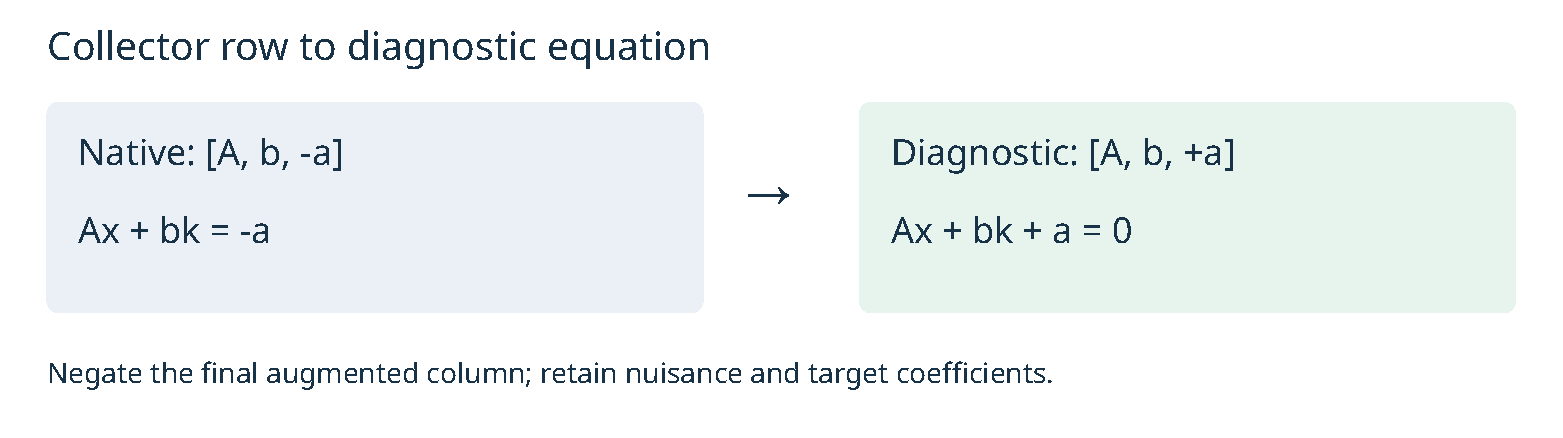
\includegraphics[width=\textwidth]{correspondence.pdf}

\textbf{Implementation.} A separate offline adapter validates the prime-field domain and row widths, reduces coefficients, and negates only the final augmented column. Rank and consistency predicates are unchanged by this nonzero column scaling, but concrete solution interpretation now agrees with the signed equation.

\textbf{Fixed controls.} Three native release tests passed. One fixture reconstructs the unique assignment $(x,k)=(2,3)$ over $\mathbf F_7$. Exhaustive checks cover all 343 single-row augmented systems over $\mathbf F_7$ and all 49 assignments for each, comparing the original right-hand-side equation to the converted zero equation. Wrong domains, widths, overflowing column counts and noncanonical inputs are checked. Strict Clippy passed.

\textbf{Scope.} This is an adapter for supplied rows, not production trace capture. It performs additional elimination and copies outside measured collection. It provides no historical per-relation costs, collection-policy timing or cohort result. Independent source review is pending in a separate packet. Future ingestion must bind actual producer source, scalar modulus, column identities, admission status and phase-cost records.

\textbf{Reproduction.} The source manifest binds the native producer, original information diagnostic and adapter. The frozen test plan, exact commands and native exit receipts accompany this report. Existing full 1,260-target evaluation requirements remain unchanged.
\end{document}